\section{Zagrożenia}
\begin{frame}{Zagrożenia}
    \begin{block}{Co może się wydarzyć?}
    \begin{itemize}
      \item Kradzież tożsamości
      \item Naruszenie prywatności i poufności danych
      \item Cyberstalking i nękanie
      \item Oszustwa socjotechniczne i internetowe
      \item Konsekwencje reputacyjne
      \item Odpowiedzialność prawna
    \end{itemize}
    \end{block}
\end{frame}

\begin{frame}{}
  \begin{center}
    {\huge Przykłady z życia}
  \end{center}
\end{frame}

\begin{frame}{Oferta sprzedaży bazy klientów Empiku}
\begin{columns}[c]
    \column{.5\textwidth}
    \begin{block}{}
      \begin{itemize}
        \item Marzec 2025
        \item Ogłoszenie dotyczące sprzedaży rzekomej bazy danych zawierającej informacje o 24 milionach klientów Empiku
        \item Baza miała zawierać takie dane jak: imię i nazwisko, numer telefonu, adresy i informacje o zamówieniach
      \end{itemize}
      \end{block}
    \begin{exampleblock}{Empik: reakcja}
    \begin{itemize}
      \item Szybka analiza
      \item Komunikacja z klientami
      \item Współpraca z zespołem CERT \cite{empik}
    \end{itemize}
    \end{exampleblock}
    \column{.5\textwidth}
    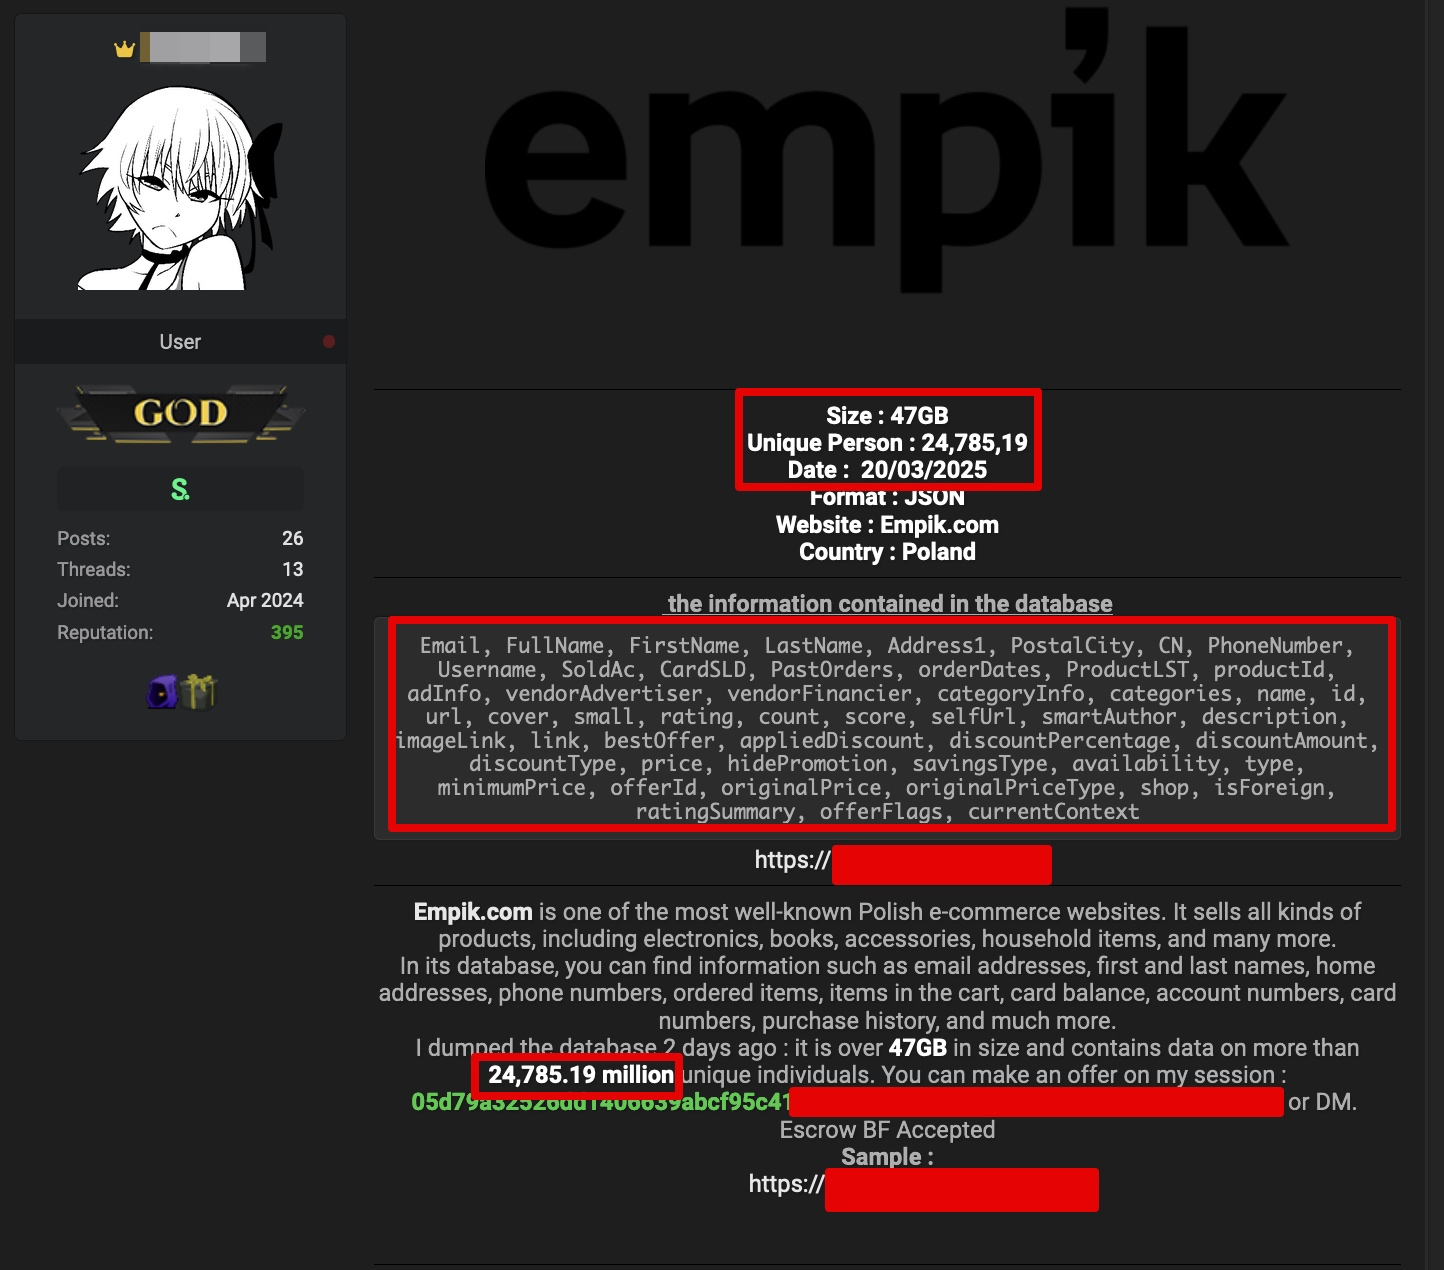
\includegraphics[width=1\textwidth]{images/empik-wyciek.jpg}
\end{columns}
\end{frame}

\begin{frame}{Fałszywe oskarżenie o pedofilię i złodziejstwo}
\begin{columns}[c]
    \column{.55\textwidth}
    \begin{itemize}
      \item Phishing
      \item Kradzież tożsamości
      \item Strach o karierę i reputację
    \end{itemize}
    \column{.45\textwidth}
    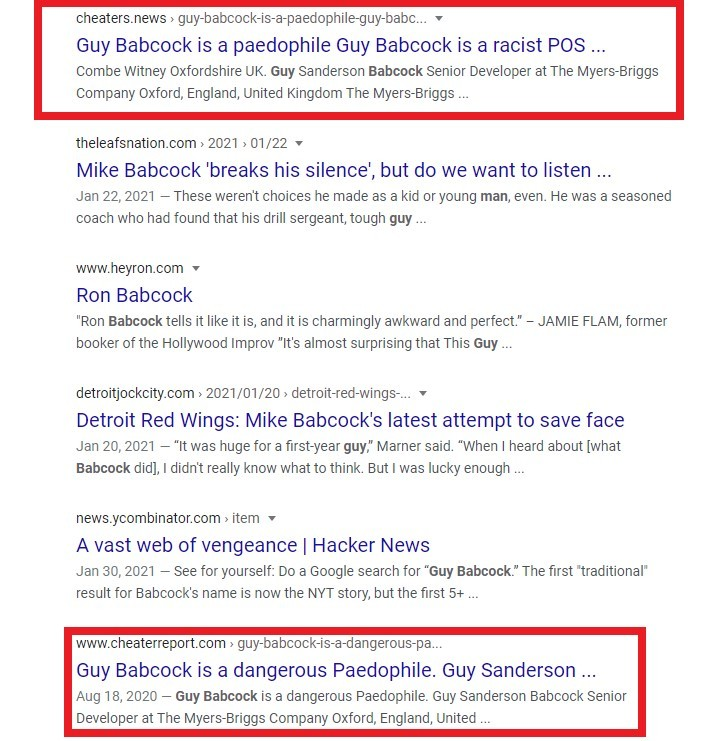
\includegraphics[width=1\textwidth]{images/pedophile.jpg}
\end{columns}
\end{frame}

\begin{frame}{Nękanie i wandalizm}
\begin{columns}[c]
    \column{.65\textwidth}
    \begin{block}{}
      W styczniu 2021 roku senator Mitch McConnell spotkał się z falą krytyki po tym, jak zablokował propozycję zwiększenia kwoty wypłat w ramach rządowej pomocy COVID-19.
    \end{block}
    \column{.35\textwidth}
    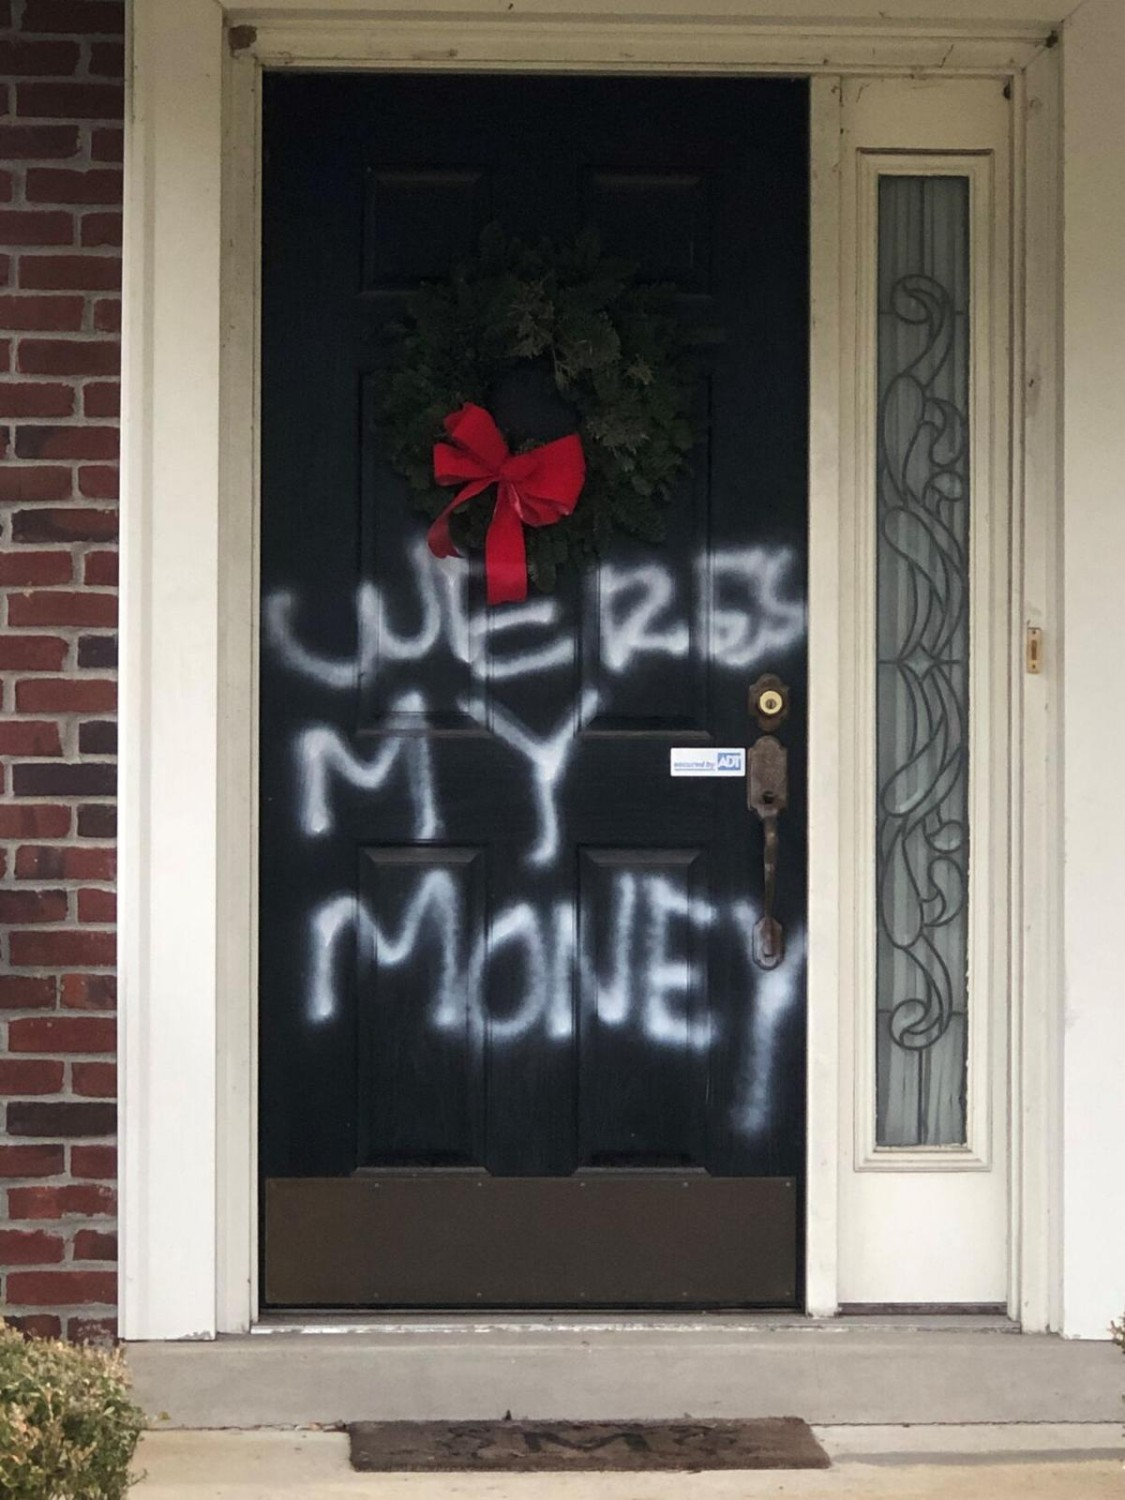
\includegraphics[width=1\textwidth]{images/vandalism.jpg}
\end{columns}
\end{frame}

\begin{frame}{Odpowiedzialność prawna}
    \begin{columns}[c]
      \column{.75\textwidth}
      \begin{block}{}
        Japończyk Hibiki Sato użył zdjęć z mediów społecznościowych i na podstawie refleksów w oczach i Google Street View, by odnaleźć kobietę i ją zaatakować.
      \end{block}
      \column{.25\textwidth}
      
\includegraphics[width=1\textwidth]{images/law.png}
  \end{columns}
\end{frame}